\documentclass[aspectratio=169, 9pt]{beamer}

% Pacotes de codificação e idioma
\usepackage[utf8]{inputenc}
\usepackage[T1]{fontenc}
\usepackage[brazil]{babel}
\usepackage{lmodern}

% Pacotes matemáticos e científicos
\usepackage{amsmath, amssymb, amsfonts}
\usepackage{mathtools}
\usepackage{bm}

% Pacotes gráficos e de layout
\usepackage{graphicx}
\usepackage{booktabs}
\usepackage{array}
\usepackage{tikz}
\usetikzlibrary{shapes.geometric, arrows.meta, positioning, calc}

% Tema e paleta de cores
\usetheme{Madrid}
\usecolortheme{whale}
\usefonttheme{professionalfonts}

% Cores personalizadas (Azul Escuro Acadêmico e Vermelho Thorlabs/Laser)
\definecolor{PrimaryBlue}{RGB}{15, 45, 90}
\definecolor{SecondaryBlue}{RGB}{30, 85, 150}
\definecolor{LaserRed}{RGB}{185, 25, 35}
\definecolor{LightBg}{RGB}{242, 246, 252}
\definecolor{AlertBg}{RGB}{253, 242, 242}
\definecolor{DarkText}{RGB}{30, 35, 45}

\setbeamercolor{palette primary}{bg=PrimaryBlue, fg=white}
\setbeamercolor{palette secondary}{bg=SecondaryBlue, fg=white}
\setbeamercolor{palette tertiary}{bg=PrimaryBlue!90!black, fg=white}
\setbeamercolor{palette quaternary}{bg=PrimaryBlue, fg=white}
\setbeamercolor{structure}{fg=PrimaryBlue}
\setbeamercolor{title}{fg=white, bg=PrimaryBlue}
\setbeamercolor{frametitle}{fg=white, bg=PrimaryBlue}
\setbeamercolor{block title}{bg=SecondaryBlue, fg=white}
\setbeamercolor{block body}{bg=LightBg, fg=DarkText}
\setbeamercolor{block title alerted}{bg=LaserRed, fg=white}
\setbeamercolor{block body alerted}{bg=AlertBg, fg=DarkText}
\setbeamercolor{block title example}{bg=PrimaryBlue!85!teal, fg=white}
\setbeamercolor{block body example}{bg=LightBg, fg=DarkText}

% Remoção de símbolos de navegação e ajuste de margens
\setbeamertemplate{navigation symbols}{}
\setbeamertemplate{itemize items}[circle]
\setbeamertemplate{enumerate items}[default]
\setbeamersize{text margin left=5.5mm, text margin right=5.5mm}

% Rodapé customizado
\setbeamertemplate{footline}{
  \leavevmode%
  \hbox{%
  \begin{beamercolorbox}[wd=.333333\paperwidth,ht=2.25ex,dp=1ex,center]{author in head/foot}%
    \usebeamerfont{author in head/foot}Equipe 4: Logan e Samuel Farias
  \end{beamercolorbox}%
  \begin{beamercolorbox}[wd=.444444\paperwidth,ht=2.25ex,dp=1ex,center]{title in head/foot}%
    \usebeamerfont{title in head/foot}Cap. 8: Materiais e Dispositivos Optoeletrônicos
  \end{beamercolorbox}%
  \begin{beamercolorbox}[wd=.222222\paperwidth,ht=2.25ex,dp=1ex,right]{date in head/foot}%
    \usebeamerfont{date in head/foot}Slide \insertframenumber{} / \inserttotalframenumber\hspace*{2ex}
  \end{beamercolorbox}}%
  \vskip0pt%
}

% Metadados da Apresentação
\title[Tema 4: Optoeletrônica e Fotodetectores]{\textbf{Capítulo 8: Materiais e Dispositivos Optoeletrônicos}}
\subtitle{Revisão Teórica (8.1 a 8.4) e Caracterização Experimental da Responsividade do Fotodiodo InGaAs (SM05PD5A)}
\author[Equipe 4: Logan e Samuel Farias]{\textbf{Equipe 4:} Logan e Samuel Farias}
\institute[Materiais Eletrônicos e Optoeletrônicos]{%
  Disciplina: Materiais Eletrônicos e Optoeletrônicos $\bullet$ 2ª Avaliação --- Seminários
}
\date{Novembro / Dezembro de 2026}

\begin{document}
\setlength{\abovedisplayskip}{3pt}
\setlength{\belowdisplayskip}{3pt}

% ============================================================================
% SLIDE 1: CAPA E VISÃO GERAL
% ============================================================================
\begin{frame}
  \vspace{-0.2cm}
  \titlepage
  \vspace{-0.45cm}
  \begin{columns}[T, onlytextwidth]
    \begin{column}{0.485\textwidth}
      \begin{block}{\footnotesize Parte I: Revisão Teórica (Slides 2--5)}
        \scriptsize
        \textbf{8.1} Propriedades Ópticas $\bullet$ \textbf{8.2} Modelo Clássico (Drude e Lorentz) $\bullet$ \textbf{8.3} Teoria Quântica e \textit{Gap} $\bullet$ \textbf{8.4} Fotodetectores e Responsividade.
      \end{block}
    \end{column}
    \begin{column}{0.485\textwidth}
      \begin{alertblock}{\footnotesize Parte II: Experimento e Resultados (Slides 6--10)}
        \scriptsize
        Caracterização de $\mathcal{R}(\lambda)$ no \textbf{SM05PD5A} ($\text{InGaAs}$) com lasers \textbf{MCLS1} ($1350\text{ nm}$ e $1550\text{ nm}$), módulo \textbf{PBM42} e vídeo demonstrativo.
      \end{alertblock}
    \end{column}
  \end{columns}
  \vspace{0.1cm}
  \begin{center}
    \scriptsize \textcolor{SecondaryBlue}{\textbf{Referências:} S. M. Rezende, \textit{Materiais e Dispositivos Eletrônicos}, 2ª Ed. (Cap. 8) $\bullet$ Datasheets Thorlabs (MCLS1, SM05PD5A, PBM42)}
  \end{center}
\end{frame}

% ============================================================================
% SLIDE 2: [TEORIA 1/4] 8.1 PROPRIEDADES ÓPTICAS DOS MATERIAIS
% ============================================================================
\begin{frame}{8.1 Propriedades Ópticas dos Materiais}
  \begin{columns}[T, onlytextwidth]
    \begin{column}{0.49\textwidth}
      \begin{block}{Equação de Onda e Índice Complexo}
        Em um meio com permissividade $\varepsilon$ e condutividade $\sigma$, as equações de Maxwell levam a:
        \[
          \frac{\partial^2 \vec{\mathcal{E}}}{\partial x^2} = \mu\varepsilon \frac{\partial^2 \vec{\mathcal{E}}}{\partial t^2} + \mu\sigma \frac{\partial \vec{\mathcal{E}}}{\partial t}
        \]
        A propagação é descrita pelo \textbf{índice de refração complexo} $N(\omega)$:
        \[
          N(\omega) = \left(\varepsilon + i\frac{\sigma}{\omega\varepsilon_0}\right)^{1/2} = n + i\kappa
        \]
        \begin{itemize}
          \item $n = c/v_f$: \textbf{índice de refração} (define a velocidade de fase no meio).
          \item $\kappa$: \textbf{coeficiente de extinção} (determina a atenuação da onda).
        \end{itemize}
      \end{block}
    \end{column}

    \begin{column}{0.48\textwidth}
      \begin{alertblock}{Absorção e Lei de Beer-Lambert}
        A amplitude decai como $e^{-\frac{\omega\kappa}{c}x}$ e a intensidade média ($I \propto \mathcal{E}_0^2$) decai exponencialmente:
        \[
          I(x) = I_0 \, e^{-\alpha x}, \qquad \alpha = \frac{2\omega\kappa}{c} = \frac{4\pi\kappa}{\lambda}
        \]
        \begin{itemize}
          \item $\alpha$: \textbf{coeficiente de absorção} ($\text{m}^{-1}$ ou $\text{cm}^{-1}$); profundidade $\delta = 2/\alpha$.
          \item \textbf{Fluxo de fótons:} $\Phi = \dfrac{I}{\hbar\omega} = \dfrac{P}{A\,\hbar\omega} = \dfrac{P\,\lambda}{A\,hc}$.
        \end{itemize}
      \end{alertblock}
      \vspace{-0.1cm}
      \begin{exampleblock}{Refletividade Normal ($R$, com $R + T = 1$)}
        \[
          R = \frac{(n-1)^2 + \kappa^2}{(n+1)^2 + \kappa^2}
        \]
      \end{exampleblock}
    \end{column}
  \end{columns}
\end{frame}

% ============================================================================
% SLIDE 3: [TEORIA 2/4] 8.2 INTERAÇÃO DA RADIAÇÃO COM A MATÉRIA - MODELO CLÁSSICO
% ============================================================================
\begin{frame}[shrink=2]{8.2 Interação da Radiação com a Matéria --- Modelo Clássico}
  \begin{columns}[T, onlytextwidth]
    \begin{column}{0.485\textwidth}
      \begin{block}{8.2.1 Elétrons Livres em Metais (Drude)}
        Com tempo médio de colisão $\tau$:
        \[
          m\frac{dv}{dt} + \frac{m}{\tau}v = -e\mathcal{E}_0 e^{-i\omega t} \;\Rightarrow\; \sigma(\omega) = \frac{Ne^2\tau}{m(1 - i\omega\tau)}
        \]
        Para altas frequências ($\omega\tau \gg 1$):
        \[
          N^2(\omega) = \varepsilon_c\left(1 - \frac{\omega_p^2}{\omega^2}\right), \quad \omega_p^2 = \frac{Ne^2}{m\varepsilon_0\varepsilon_c}
        \]
        \begin{itemize}
          \item $\omega_p$: \textbf{frequência de plasma} ($\hbar\omega_p \sim 4\text{--}10\text{ eV}$, UV).
          \item $\omega < \omega_p$ (IR/Visível): $N$ imaginário puro ($n = 0 \Rightarrow \mathbf{R = 1}$, alta refletividade metálica).
          \item $\omega > \omega_p$ (UV): $N$ real (meio transparente).
        \end{itemize}
      \end{block}
    \end{column}

    \begin{column}{0.485\textwidth}
      \begin{block}{8.2.2 Elétrons Ligados (Oscilador de Lorentz)}
        Elétrons sujeitos à força restauradora ($m\omega_0^2 x$) e amortecimento $\Gamma$:
        \[
          m\left(\frac{d^2x}{dt^2} + \Gamma\frac{dx}{dt} + \omega_0^2 x\right) = -e\mathcal{E}_0 e^{-i\omega t}
        \]
        Da polarização $P = -Nex$ obtém-se $\varepsilon(\omega) = \varepsilon'(\omega) + i\varepsilon''(\omega)$:
        \[
          \varepsilon''(\omega) = \frac{\omega_p^2\,\omega\Gamma}{(\omega_0^2 - \omega^2)^2 + \omega^2\Gamma^2} \approx \frac{\pi\omega_p^2}{2\omega_0} f_L(\omega)
        \]
        \begin{itemize}
          \item \textbf{Ressonância ($\omega \approx \omega_0$):} Pico Lorentziano de absorção ($\varepsilon''$) associado à dispersão em $\varepsilon'(\omega)$ (Kramers-Kronig).
        \end{itemize}
      \end{block}
      \vspace{-0.15cm}
      \begin{alertblock}{Limite Clássico}
        \scriptsize Não explica o corte abrupto de absorção em $E_g$ nos semicondutores $\rightarrow$ requer descrição quântica (Seção 8.3).
      \end{alertblock}
    \end{column}
  \end{columns}
\end{frame}

% ============================================================================
% SLIDE 4: [TEORIA 3/4] 8.3 TEORIA QUÂNTICA DA INTERAÇÃO RADIAÇÃO-MATÉRIA
% ============================================================================
\begin{frame}[shrink=7]{8.3 Teoria Quântica da Interação Radiação-Matéria}
  \begin{columns}[T, onlytextwidth]
    \begin{column}{0.56\textwidth}
      \begin{block}{Transições Quânticas (Regra de Ouro de Fermi)}
        A perturbação de dipolo elétrico $\mathcal{H}' = -\mathcal{E}p_y e^{-i\omega t}$ induz transições $E_1 \to E_2$ com taxa:
        \[
          W_{12} = \frac{2\pi}{\hbar}\mathcal{E}^2 p_{12}^2 D(E_2 - E_1 - \hbar\omega)
        \]
        Exige $\hbar\omega = E_2 - E_1$, $p_{12} \neq 0$ e $N_1 > N_2$.
      \end{block}
      \vspace{-0.15cm}
      \begin{alertblock}{Transições Interbanda em Semicondutores}
        \begin{itemize}
          \item \textbf{Condição de absorção:} $\hbar\omega \ge E_g$ (abaixo de $E_g$, o material é transparente).
          \item \textbf{Comprimento de onda de corte ($\lambda_g$):}
          \[
            \lambda \le \lambda_g = \frac{hc}{E_g} \implies \mathbf{\lambda_g\,(\mu\text{m}) \approx \frac{1{,}24}{E_g\,(\text{eV})}}
          \]
          \item \textbf{Gap Direto} ($\text{GaAs}, \text{InP}, \text{InGaAs}$): $\vec{k}_f \simeq \vec{k}_i$, absorção forte $\alpha \propto (\hbar\omega - E_g)^{1/2}/\omega$.
          \item \textbf{Gap Indireto} ($\text{Si}, \text{Ge}$): exige participação de um \textbf{fônon} ($\hbar\Omega, \vec{q}$).
        \end{itemize}
      \end{alertblock}
    \end{column}

    \begin{column}{0.41\textwidth}
      \begin{center}
        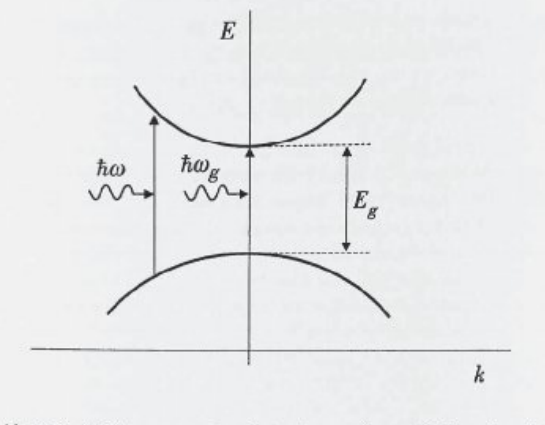
\includegraphics[height=2.35cm]{figuras/rezende_gap_direto.png}\\
        {\scriptsize \textbf{Fig. 8.8 (Rezende):} Absorção em \textit{gap} direto ($\hbar\omega \ge E_g$).}
      \end{center}
      \vspace{-0.15cm}
      \begin{table}
        \centering
        \scriptsize
        \begin{tabular}{lccc}
          \toprule
          \textbf{Material} & \textbf{Gap} & $E_g$ (eV) & $\lambda_g$ ($\mu$m) \\
          \midrule
          $\text{Si}$ & Indireto & $1{,}12$ & $1{,}11$ \\
          $\text{Ge}$ & Indireto & $0{,}67$ & $1{,}88$ \\
          $\text{GaAs}$ & Direto & $1{,}43$ & $0{,}86$ \\
          $\text{InP}$ & Direto & $1{,}35$ & $0{,}92$ \\
          \textbf{InGaAs} & \textbf{Direto} & $\mathbf{0{,}73}$ & $\mathbf{1{,}70}$ \\
          \bottomrule
        \end{tabular}
      \end{table}
      \vspace{-0.2cm}
      {\scriptsize \textcolor{LaserRed}{\textbf{Nota:}} O $\text{Si}$ corta em $1{,}11\,\mu\text{m}$; para $1350/1550\text{ nm}$ usa-se $\text{InGaAs}$.}
    \end{column}
  \end{columns}
\end{frame}

% ============================================================================
% SLIDE 5: [TEORIA 4/4] 8.4 FOTODETECTORES E FOTODIODOS
% ============================================================================
\begin{frame}[shrink=3]{8.4 Fotodetectores, Junção $p\text{-}n$ e Responsividade}
  \begin{columns}[T, onlytextwidth]
    \begin{column}{0.56\textwidth}
      \begin{block}{Princípios e Principais Dispositivos}
        Para absorção eficiente, requer-se espessura ativa $d \gg \alpha^{-1}$ ($\alpha \sim 10^6\text{ m}^{-1}$). A \textbf{eficiência quântica} $\eta \in [0,1]$ mede os pares elétron-buraco coletados por fóton incidente.
        \begin{itemize}
          \item \textbf{Tipos:} Foto-resistores (LDR, alto ganho, lentos $\sim 50\text{ ms}$), \textbf{Fotodiodos} ($p\text{-}n$/PIN/Avalanche, rápidos $\sim\text{ns}$), Células Solares e CCDs.
        \end{itemize}
      \end{block}
      \vspace{-0.1cm}
      \begin{exampleblock}{Fotodiodo $p\text{-}n$: Modos de Operação}
        \[
          I = I_s\left(e^{eV/k_B T} - 1\right) - I_L, \qquad I_L = \frac{\eta \, e \, P_L \, \lambda}{hc}
        \]
        \begin{itemize}
          \item \textbf{Fotovoltaico ($I=0$):} gera tensão $V_{ca}$; corrente de escuro mínima.
          \item \textbf{Fotocondutivo ($V < 0$, Polarização Reversa):} usado no experimento; reduz $C_J$, aumenta velocidade e garante \textbf{linearidade} ($I_L \propto P_L$).
        \end{itemize}
      \end{exampleblock}
    \end{column}

    \begin{column}{0.41\textwidth}
      \begin{center}
        \begin{columns}[c, onlytextwidth]
          \begin{column}{0.49\textwidth}
            \centering
            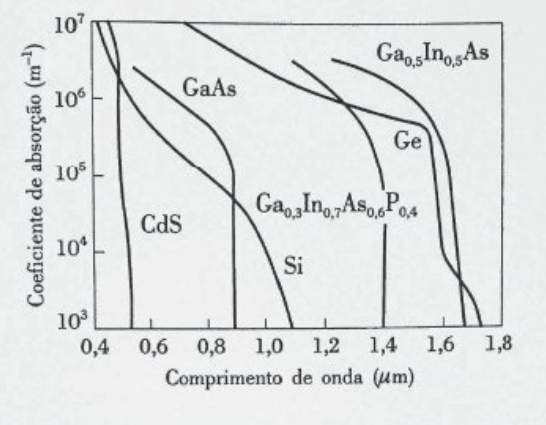
\includegraphics[height=2.15cm]{figuras/rezende_absorcao.png}\\
            {\tiny \textbf{Fig. 8.15:} $\alpha(\lambda)$ por material.}
          \end{column}
          \begin{column}{0.49\textwidth}
            \centering
            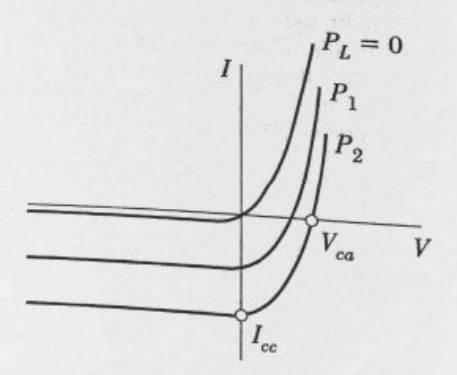
\includegraphics[height=2.15cm]{figuras/rezende_curva_iv.png}\\
            {\tiny \textbf{Fig. 8.20:} Curva $I\text{--}V$ iluminada.}
          \end{column}
        \end{columns}
      \end{center}
      \vspace{0.05cm}
      \begin{alertblock}{Responsividade $\mathcal{R}(\lambda)$ [A/W]}
        Razão entre fotocorrente ($I_P \equiv I_L$) e potência óptica ($P$):
        \[
          \mathbf{\mathcal{R}(\lambda) = \frac{I_P}{P} = \frac{\eta \, e \, \lambda}{hc} \approx \eta\,\frac{\lambda\,(\mu\text{m})}{1{,}24}\;\text{[A/W]}}
        \]
        \scriptsize Para potência $P$ fixa, $\lambda$ maior fornece mais fótons/s ($\Phi = P\lambda/hc$), elevando $\mathcal{R}(\lambda)$.
      \end{alertblock}
    \end{column}
  \end{columns}
\end{frame}

% ============================================================================
% SLIDE 6: [EXPERIMENTO 1/5] ARRANJO EXPERIMENTAL E EQUIPAMENTOS
% ============================================================================
\begin{frame}[shrink=2]{Parte Experimental: Arranjo e Equipamentos}
  \begin{center}
    \begin{tikzpicture}[
      box/.style={rectangle, rounded corners=4pt, draw=PrimaryBlue, very thick, fill=LightBg, text width=2.65cm, align=center, minimum height=1.25cm, font=\scriptsize\sffamily},
      laserbox/.style={rectangle, rounded corners=4pt, draw=LaserRed, very thick, fill=AlertBg, text width=2.75cm, align=center, minimum height=1.25cm, font=\scriptsize\sffamily},
      arrow/.style={-{Stealth[length=2.1mm, width=1.6mm]}, very thick, color=PrimaryBlue},
      optarrow/.style={-{Stealth[length=2.1mm, width=1.6mm]}, very thick, color=LaserRed, dashed}
    ]
      \node[laserbox] (mcls) {\textbf{Fonte Laser MCLS1}\\Lasers Diodo em Fibra\\$\lambda_1 = 1350\text{ nm}$ e $\lambda_2 = 1550\text{ nm}$};
      \node[box, right=0.95cm of mcls] (pd) {\textbf{Fotodiodo SM05PD5A}\\Sensor $\text{InGaAs}$\\Área: $3{,}1\text{ mm}^2$ ($\varnothing\,2{,}0\text{ mm}$)};
      \node[box, right=0.95cm of pd] (pbm) {\textbf{Módulo PBM42}\\Polarização Reversa\\($V_R \le 3\text{ V}$) + Filtro RC};
      \node[box, right=0.95cm of pbm] (meas) {\textbf{Carga $R_L$ e Leitura}\\Medição de $V_o$ ou $I_P$\\$\mathcal{R}(\lambda) = I_P / P$};

      \draw[optarrow] (mcls) -- node[above, font=\scriptsize\bfseries, color=LaserRed] {Fibra} node[below, font=\tiny, color=LaserRed] {$P$} (pd);
      \draw[arrow] (pd) -- node[above, font=\scriptsize\bfseries] {BNC} node[below, font=\tiny] {$I_P(\lambda)$} (pbm);
      \draw[arrow] (pbm) -- node[above, font=\scriptsize\bfseries] {SMA} node[below, font=\tiny] {Sinal CC} (meas);
    \end{tikzpicture}
  \end{center}
  \vspace{-0.1cm}
  \begin{columns}[T, onlytextwidth]
    \begin{column}{0.53\textwidth}
      \begin{block}{Especificações dos Componentes (Datasheets)}
        \scriptsize
        \begin{itemize}
          \item \textbf{Fonte Thorlabs MCLS1:} 4 canais acoplados a fibra (\texttt{FC/PC}), controle de corrente ($0{,}01\text{ mA}$) e TEC ($20\text{--}30\,^\circ\text{C}$, $\pm 0{,}01\,^\circ\text{C}$). Precisão do visor: $\pm 10\%$. Laser Classe 3B (\textit{Keylock}, \textit{Interlock}, delay $3\text{ s}$).
          \item \textbf{Fotodiodo SM05PD5A ($\text{InGaAs}$):} faixa $800\text{--}1700\text{ nm}$, pico $\mathcal{R}(1590\text{ nm}) = 1{,}04\text{ A/W}$, cátodo aterrado, $C_J = 100\text{ pF}$, $I_d = 50\text{ nA}$ ($1\text{ V}$), \textbf{máx. $V_R = 3\text{ V}$}.
          \item \textbf{Módulo PBM42:} aplica $V_R$ (pino central positivo para cátodo aterrado) via filtro RC ($1\text{ k}\Omega$, $0{,}1\,\mu\text{F}$).
        \end{itemize}
      \end{block}
    \end{column}

    \begin{column}{0.44\textwidth}
      \begin{center}
        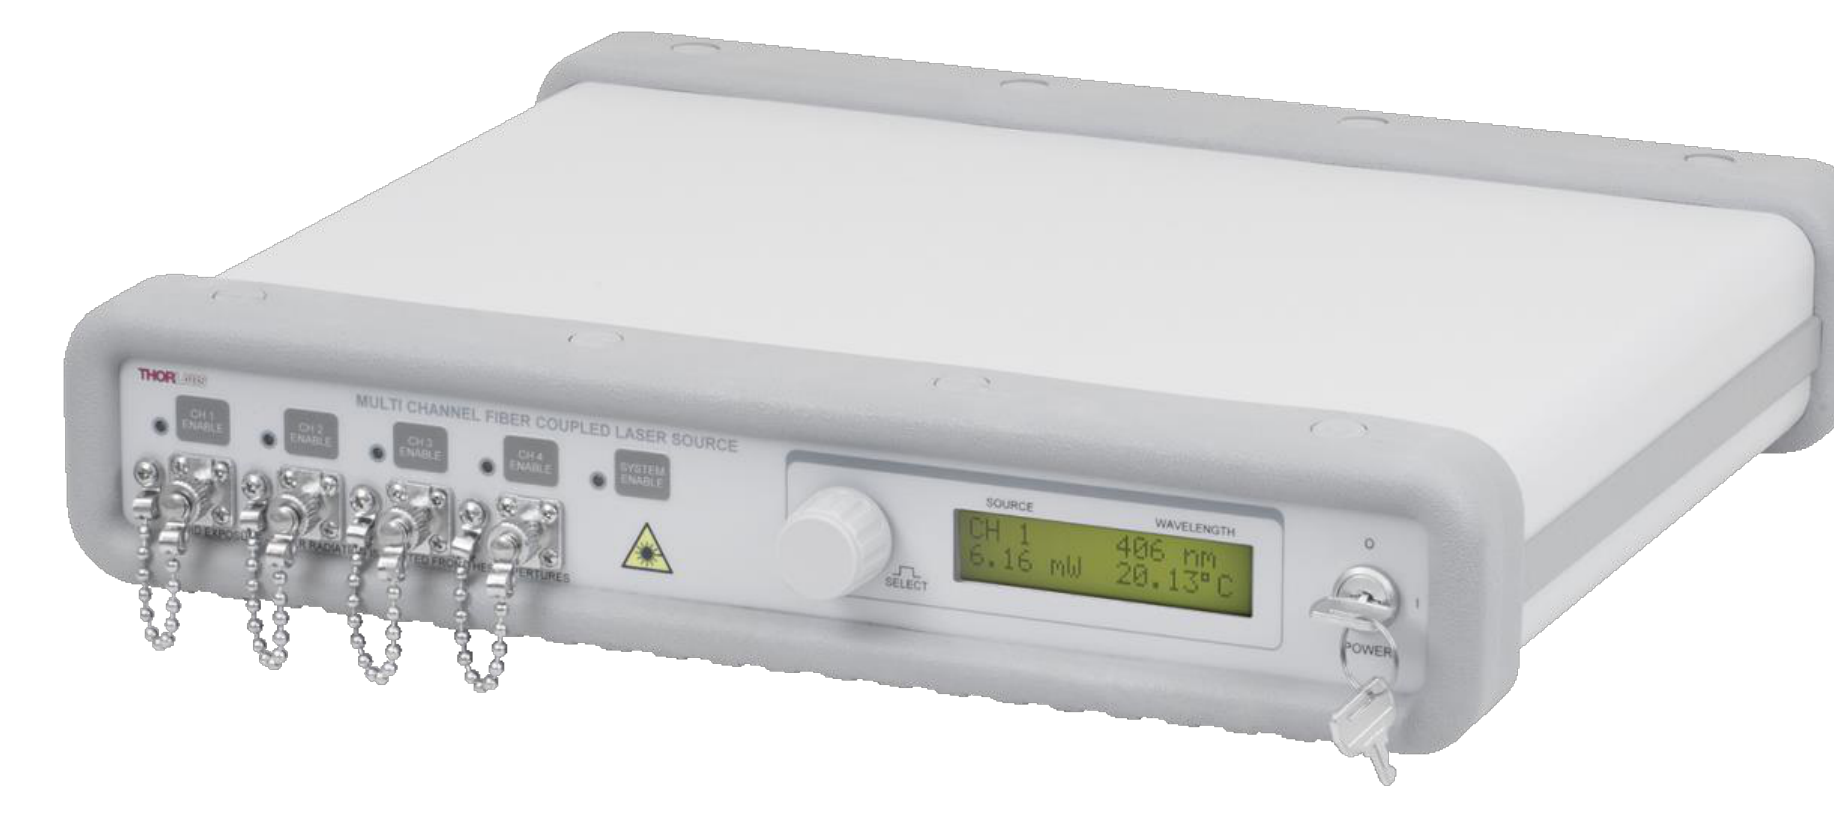
\includegraphics[height=1.85cm]{figuras/mcls1_foto.png}\\[2pt]
        {\tiny \textbf{Fonte Multicanal MCLS1}}
        \vspace{0.1cm}
        \begin{columns}[c, onlytextwidth]
          \begin{column}{0.48\textwidth}
            \centering
            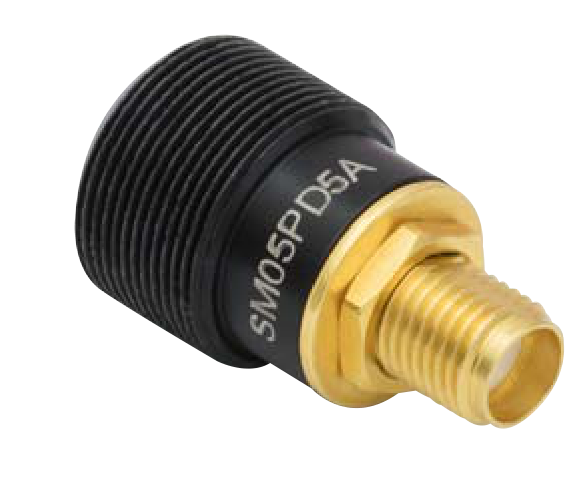
\includegraphics[height=1.55cm]{figuras/sm05pd5a_foto.png}\\
            {\tiny \textbf{SM05PD5A}}
          \end{column}
          \begin{column}{0.48\textwidth}
            \centering
            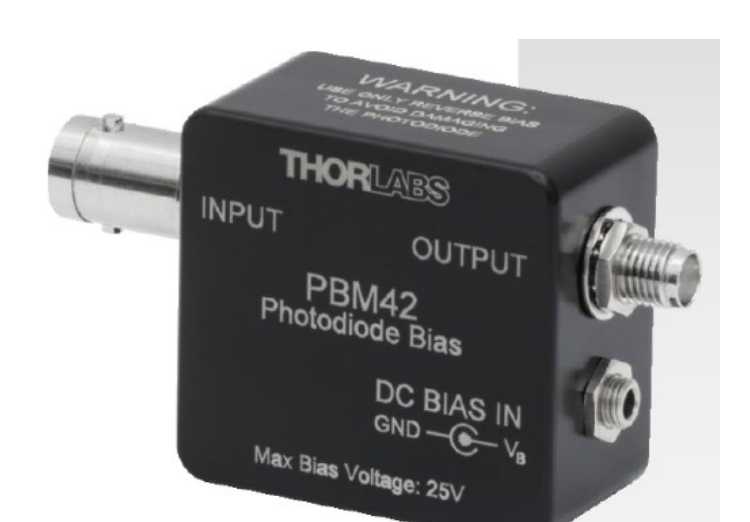
\includegraphics[height=1.55cm]{figuras/pbm42_foto.png}\\
            {\tiny \textbf{PBM42}}
          \end{column}
        \end{columns}
      \end{center}
    \end{column}
  \end{columns}
\end{frame}

% ============================================================================
% SLIDE 7: [EXPERIMENTO 2/5] CIRCUITO, PROCEDIMENTO E EXIBIÇÃO DO VÍDEO
% ============================================================================
\begin{frame}[shrink=2]{Circuito de Leitura, Procedimento e Vídeo do Experimento}
  \begin{columns}[T, onlytextwidth]
    \begin{column}{0.51\textwidth}
      \begin{block}{Circuito Equivalente e Equações de Medição}
        A fotocorrente $I_P$ percorre o resistor de carga $R_L$, gerando $V_o$:
        \[
          V_o = I_P \cdot R_L = P \cdot \mathcal{R}(\lambda) \cdot R_L \implies \mathcal{R}(\lambda) = \frac{V_o}{P \cdot R_L}
        \]
        \begin{itemize}
          \item \textbf{Condição de operação:} manter $V_o \ll V_R$ ($V_R \le 3\text{ V}$) para preservar a polarização reversa e a linearidade.
          \item \textbf{Banda dinâmica:} $f_{BW} = \frac{1}{2\pi R_L C_J}$ (em CC/CW, $R_L$ maior amplia $V_o$ sem comprometer a medida estática).
        \end{itemize}
        \begin{center}
          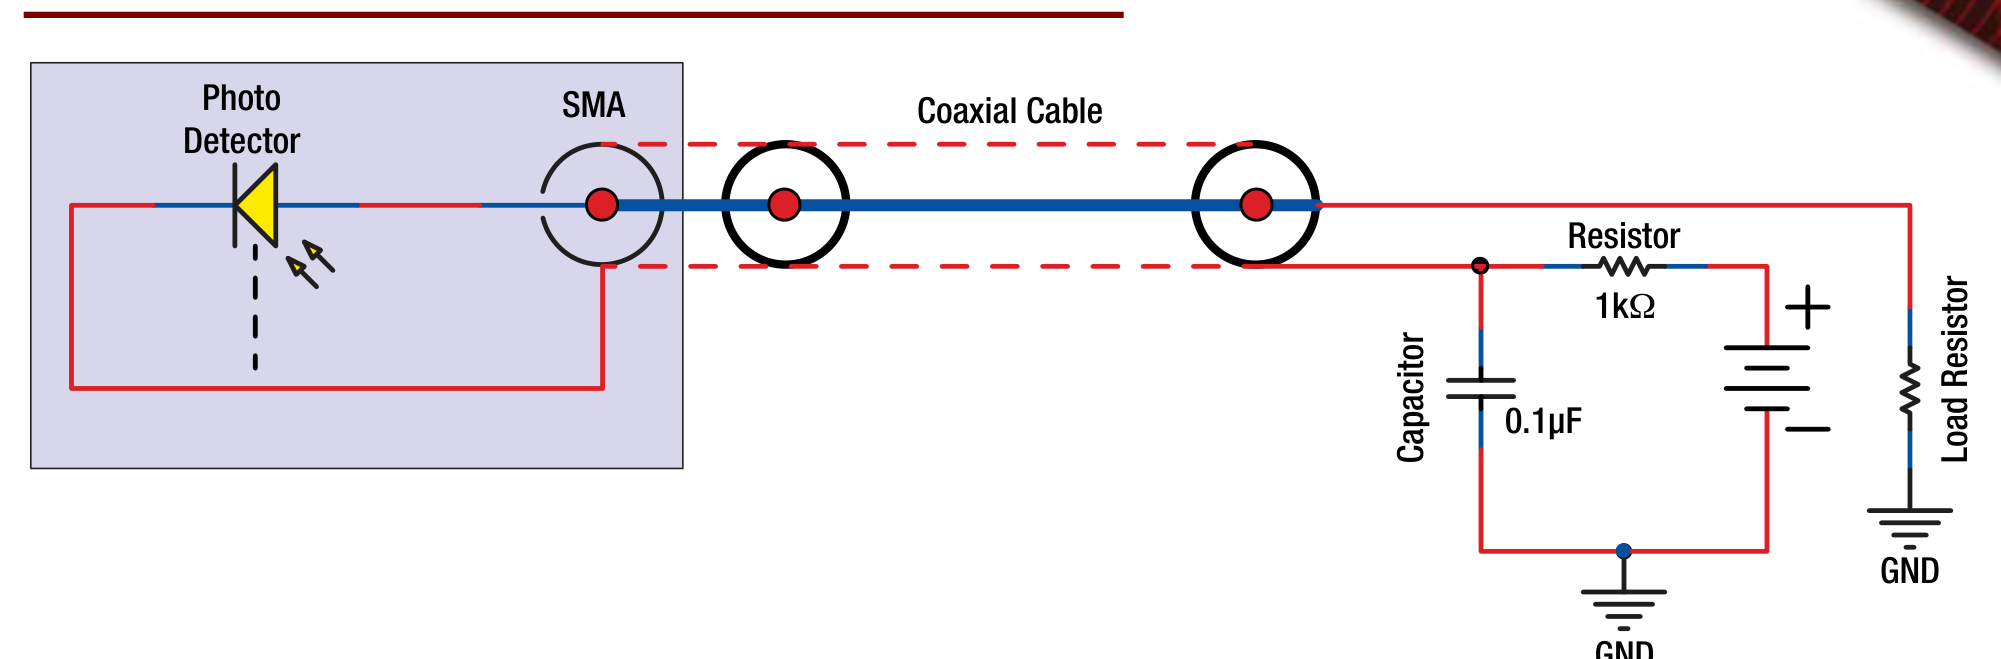
\includegraphics[width=0.90\textwidth]{figuras/sm05pd5a_circuito.png}
        \end{center}
      \end{block}
    \end{column}

    \begin{column}{0.46\textwidth}
      \begin{exampleblock}{Roteiro Experimental Adotado}
        \begin{enumerate}
          \item Polarizar reversamente o \textbf{SM05PD5A} via \textbf{PBM42} ($V_R = \text{[valor] V}$) e registrar o nível no escuro ($P=0$).
          \item Estabilizar o \textbf{MCLS1} em $T = 25{,}00\,^\circ\text{C}$ e acoplar a fibra ao detector.
          \item Variar a potência $P$ (múltiplos pontos) em $\lambda_1 = 1350\text{ nm}$ e registrar $V_o$ (ou $I_P$).
          \item Repetir a varredura para $\lambda_2 = 1550\text{ nm}$ e obter $\mathcal{R}_{\text{exp}}$ por ajuste linear.
        \end{enumerate}
      \end{exampleblock}
      \vspace{-0.1cm}
      \begin{alertblock}{Exibição em Sala: Vídeo do Experimento}
        \scriptsize
        \textbf{[Exibir vídeo gravado em laboratório neste momento]}
        \begin{itemize}
          \item Bancada real, ativação segura (NIR invisível), leitura no escuro e variação simultânea de $P$ e $V_o$ em $\lambda_1$ e $\lambda_2$.
          \item \textbf{Em sala:} demonstração física do conjunto \texttt{SM05PD5A + PBM42} (desligado).
        \end{itemize}
      \end{alertblock}
    \end{column}
  \end{columns}
\end{frame}

% ============================================================================
% SLIDE 8: [EXPERIMENTO 3/5] COLETA DE DADOS E LINEARIDADE I_P x P
% ============================================================================
\begin{frame}{Resultados Experimentais: Coleta e Linearidade ($I_P \times P$)}
  \begin{columns}[T, onlytextwidth]
    \begin{column}{0.51\textwidth}
      \begin{block}{Tabela de Medidas Experimentais ($T = 25{,}00\,^\circ\text{C}$)}
        \scriptsize
        Parâmetros do circuito: $V_R = \text{[X] V}$, $R_L = \text{[Y] }\Omega$, sinal no escuro $V_{o,\text{esc}} = \text{[Z] mV}$.
        \vspace{0.08cm}
        \begin{center}
          \begin{tabular}{cccc|ccc}
            \toprule
            \multicolumn{4}{c|}{\textbf{Laser 1 ($\lambda_1 = 1350\text{ nm}$)}} & \multicolumn{3}{c}{\textbf{Laser 2 ($\lambda_2 = 1550\text{ nm}$)}} \\
            $P$ & $V_o$ & $I_P$ & $\mathcal{R}_i$ & $P$ & $V_o$ & $I_P$ \\
            (mW) & (mV) & (mA) & (A/W) & (mW) & (mV) & (mA) \\
            \midrule
            \textit{---} & \textit{---} & \textit{---} & \textit{---} & \textit{---} & \textit{---} & \textit{---} \\
            \textit{---} & \textit{---} & \textit{---} & \textit{---} & \textit{---} & \textit{---} & \textit{---} \\
            \textit{---} & \textit{---} & \textit{---} & \textit{---} & \textit{---} & \textit{---} & \textit{---} \\
            \textit{---} & \textit{---} & \textit{---} & \textit{---} & \textit{---} & \textit{---} & \textit{---} \\
            \textit{---} & \textit{---} & \textit{---} & \textit{---} & \textit{---} & \textit{---} & \textit{---} \\
            \bottomrule
          \end{tabular}
        \end{center}
      \end{block}
      \vspace{-0.1cm}
      \begin{exampleblock}{Método da Regressão Linear}
        \scriptsize Ajustando $I_P = \mathcal{R}_{\text{exp}}(\lambda)\cdot P + I_0$, a inclinação fornece $\mathcal{R}_{\text{exp}}$ reduzindo desvios de \textit{offset} (corrente de escuro / luz ambiente).
      \end{exampleblock}
    \end{column}

    \begin{column}{0.46\textwidth}
      \begin{block}{Curvas Experimentais $I_P \times P$}
        \begin{center}
          \begin{tikzpicture}
            \draw[dashed, color=SecondaryBlue, fill=white, rounded corners=4pt] (0,0) rectangle (6.2,4.5);
            \node[align=center, font=\scriptsize\sffamily, color=PrimaryBlue] at (3.1,2.25) {
              \textbf{[Inserir Gráfico $I_P$ (mA) $\times$ $P$ (mW)]}\\[6pt]
              Pontos experimentais + retas ajustadas\\
              para $\lambda_1 = 1350\text{ nm}$ e $\lambda_2 = 1550\text{ nm}$\\[4pt]
              $\mathcal{R}_{\text{exp}}(1350) = \text{--- A/W}$ ($R^2 = \text{---}$)\\
              $\mathcal{R}_{\text{exp}}(1550) = \text{--- A/W}$ ($R^2 = \text{---}$)
            };
          \end{tikzpicture}
        \end{center}
      \end{block}
    \end{column}
  \end{columns}
\end{frame}

% ============================================================================
% SLIDE 9: [EXPERIMENTO 4/5] COMPARAÇÃO COM DATASHEET E ANÁLISE DE ERROS
% ============================================================================
\begin{frame}[shrink=2]{Comparação com o Datasheet e Análise de Incertezas}
  \begin{columns}[T, onlytextwidth]
    \begin{column}{0.43\textwidth}
      \begin{center}
        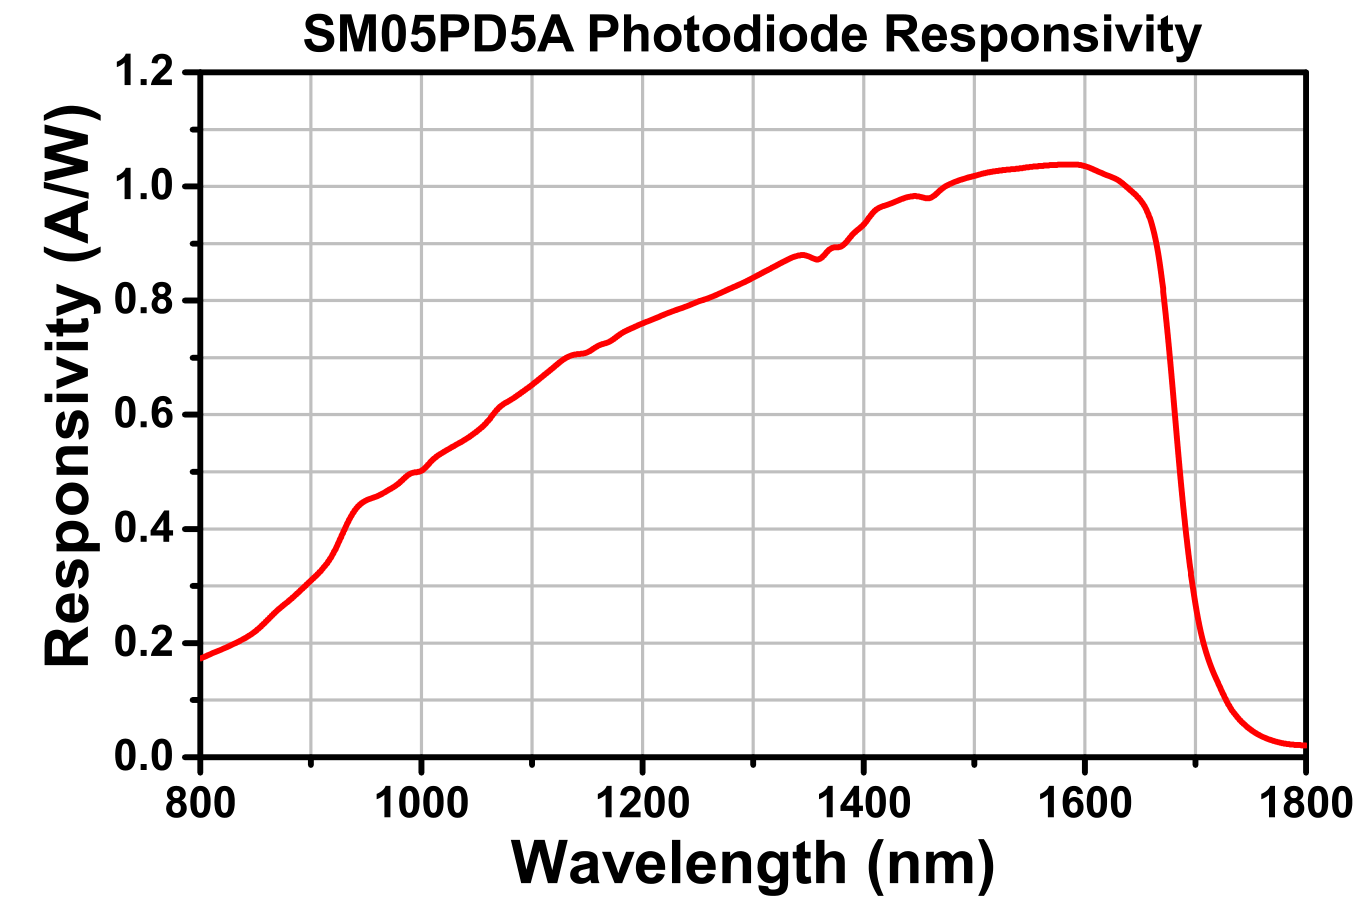
\includegraphics[width=0.95\textwidth]{figuras/sm05pd5a_responsividade.png}\\
        {\scriptsize \textbf{Curva do Fabricante (SM05PD5A):} Crescimento linear até $1590\text{ nm}$ e corte no \textit{gap} do $\text{InGaAs}$ ($\lambda_g \approx 1700\text{ nm}$).}
      \end{center}
      \vspace{-0.1cm}
      \begin{exampleblock}{Razão Esperada entre os Lasers}
        \scriptsize
        \[
          \frac{\mathcal{R}_{\text{ds}}(1550\text{ nm})}{\mathcal{R}_{\text{ds}}(1350\text{ nm})} \approx \frac{1{,}03}{0{,}88} \approx \mathbf{1{,}17}\quad (\sim 17\%\text{ maior})
        \]
        Pelo fluxo de fótons puro: $1550/1350 \approx 1{,}148$ ($+14{,}8\%$).
      \end{exampleblock}
    \end{column}

    \begin{column}{0.54\textwidth}
      \begin{block}{Síntese Comparativa: Teoria vs.\ Experimento}
        \scriptsize
        \begin{center}
          \begin{tabular}{lccccc}
            \toprule
            $\lambda$ & $E_{\text{fóton}}$ & $\mathcal{R}_{\text{ds}}$ & $\mathcal{R}_{\text{exp}}$ & Desvio & $\eta_{\text{exp}}$ \\
            (nm) & (eV) & (A/W) & (A/W) & (\%) & (\%) \\
            \midrule
            $1350$ & $0{,}919$ & $\approx 0{,}88$ & \textit{---} & \textit{---} & \textit{---} \\
            $1550$ & $0{,}800$ & $\approx 1{,}03$ & \textit{---} & \textit{---} & \textit{---} \\
            \midrule
            \textit{Razão} & --- & $\approx 1{,}17$ & \textit{---} & \textit{---} & --- \\
            \bottomrule
          \end{tabular}
        \end{center}
      \end{block}
      \vspace{-0.1cm}
      \begin{alertblock}{Principais Fontes de Erro Experimental}
        \scriptsize
        \begin{itemize}
          \item \textbf{Potência óptica ($P$):} o visor do \texttt{MCLS1} mede via fotodiodo interno com precisão de $\mathbf{\pm 10\%}$ e não contabiliza perdas nos conectores da fibra.
          \item \textbf{Acoplamento fibra--sensor:} divergência do feixe ou alinhamento fora do centro da área ativa ($\varnothing\,2{,}0\text{ mm}$) e reflexão na entrada.
          \item \textbf{Leitura elétrica:} tolerância do resistor $R_L$, resistência de contato e corrente de escuro/ruído térmico.
        \end{itemize}
      \end{alertblock}
    \end{column}
  \end{columns}
\end{frame}

% ============================================================================
% SLIDE 10: [EXPERIMENTO 5/5] CONCLUSÕES
% ============================================================================
\begin{frame}{Conclusões}
  \begin{block}{1. Seleção do Material e Teoria Quântica (Seção 8.3)}
    A detecção em $1350\text{ nm}$ e $1550\text{ nm}$ exige semicondutores de \textit{gap} estreito e direto como a liga $\text{InGaAs}$ ($E_g \approx 0{,}73\text{ eV}$, corte $\lambda_g \approx 1{,}70\,\mu\text{m}$), superando a transparência do silício ($\lambda_g \approx 1{,}11\,\mu\text{m}$) nessas janelas de telecomunicações.
  \end{block}
  \vspace{0.08cm}
  \begin{exampleblock}{2. Resposta Elétrica no Modo Fotocondutivo (Seção 8.4)}
    A polarização reversa aplicada pelo módulo \textbf{PBM42} ($V_R \le 3\text{ V}$) alarga a região de depleção e garante a proporcionalidade linear entre fotocorrente e potência óptica ($I_P = \mathcal{R}(\lambda)\,P$), validada pelas curvas experimentais.
  \end{exampleblock}
  \vspace{0.08cm}
  \begin{alertblock}{3. Confirmação Experimental da Natureza Quântica de $\mathcal{R}(\lambda)$}
    O aumento de $\mathcal{R}_{\text{exp}}$ de $1350\text{ nm}$ para $1550\text{ nm}$ comprova a relação $\mathcal{R}(\lambda) = \frac{\eta e\lambda}{hc}$: para uma mesma potência óptica incidente, fótons de menor energia ($hc/\lambda$) produzem um fluxo de fótons maior, gerando mais pares elétron-buraco por Watt.
  \end{alertblock}
\end{frame}

\end{document}
